\documentclass{standalone}
\usepackage{tikz}
\usetikzlibrary{positioning,decorations.pathreplacing,shadows.blur}
\begin{document}%
\begin{tikzpicture}%

\ifdefined\argrootsonly
   \def\drawc{1.0}
\fi

\ifdefined\argcfree
   \def\drawc{1.0}
   \def\drawcfree{1.0}
\fi

\ifdefined\argpaths
   \def\drawc{1.0}
   \def\drawcfree{1.0}
   \def\drawpaths{}
\fi

\ifdefined\argtraja
   \def\drawc{1.0}
   \def\drawcfree{1.0}
   \def\drawpaths{}
\fi

\ifdefined\argtrajb
   \def\drawc{1.0}
   \def\drawcfree{1.0}
   \def\drawtrajneighborhood{}
\fi

\ifdefined\argtrajc
   \def\drawc{1.0}
   \def\drawcfreefuzzy{}
   \def\drawtrajneighborhood{}
\fi

\ifdefined\argtrajd
   \def\drawc{1.0}
   \def\drawcfreefuzzy{}
   \def\drawtrajneighborhood{}
\fi

\ifdefined\argfirstfail
   \def\drawc{1.0}
   \def\drawcfree{1.0}
   \def\drawfirstfailtraj{}
\fi

\ifdefined\argfirstfailnext
   \def\drawc{1.0}
   \def\drawcfree{1.0}
   \def\drawfirstfailtraj{}
\fi

\ifdefined\argrrtstart
   \def\drawc{1.0}
   \def\drawcfree{1.0}
   \def\drawrrtstart{}
\fi

\ifdefined\argrrtsample
   \def\drawc{1.0}
   \def\drawcfree{1.0}
   \def\drawrrtstart{}
   \def\drawrrtsample{}
\fi

\ifdefined\argrrtcandidates
   \def\drawc{1.0}
   \def\drawcfree{1.0}
   \def\drawrrtstart{}
   \def\drawrrtsample{}
   \def\drawrrtcandidates{}
\fi

\ifdefined\argrrtchosen
   \def\drawc{1.0}
   \def\drawcfree{1.0}
   \def\drawrrtstart{}
   \def\drawrrtsample{}
   \def\drawrrtcandidates{}
\fi

\ifdefined\arggraph
   \def\drawc{1.0}
   \def\drawcfree{1.0}
   \def\drawgraph{dashed}
\fi

\ifdefined\arggraphfirst
   \def\drawgraph{dashed}
   \def\drawc{1.0}
   \def\drawcfree{1.0}
\fi

\ifdefined\arggraphfirstevaled
   \def\drawgraph{dashed}
   \def\drawc{1.0}
   \def\drawcfree{1.0}
\fi

\ifdefined\arggraphfirstnext
   \def\drawgraph{dashed}
   \def\drawc{1.0}
   \def\drawcfree{1.0}
\fi

\def\drawfadedgraph{
   \def\drawgraph{dashed}
   \def\drawc{0.2}
   \def\drawcfree{0.2}
}
\ifdefined\argastara\drawfadedgraph\fi
\ifdefined\argastarb\drawfadedgraph\fi
\ifdefined\argastarc\drawfadedgraph\fi
\ifdefined\argastard\drawfadedgraph\fi
\ifdefined\argastare\drawfadedgraph\fi
\ifdefined\argastarf\drawfadedgraph\fi
\ifdefined\argastarg\drawfadedgraph\fi
\ifdefined\argastarh\drawfadedgraph\fi
\ifdefined\argastari\drawfadedgraph\fi
\ifdefined\argastarj\drawfadedgraph\fi
\ifdefined\argastark\drawfadedgraph\fi
\ifdefined\argastarl\drawfadedgraph\fi
\ifdefined\argastarm\drawfadedgraph\fi
\ifdefined\argastarn\drawfadedgraph\fi
\ifdefined\argastaro\drawfadedgraph\fi
\ifdefined\argastarp\drawfadedgraph\fi
\ifdefined\argastarq\drawfadedgraph\fi
\ifdefined\argastarr\drawfadedgraph\fi
\ifdefined\argastars\drawfadedgraph\fi

%\node[inner sep=0] at (-3.5,1.5) {%
%   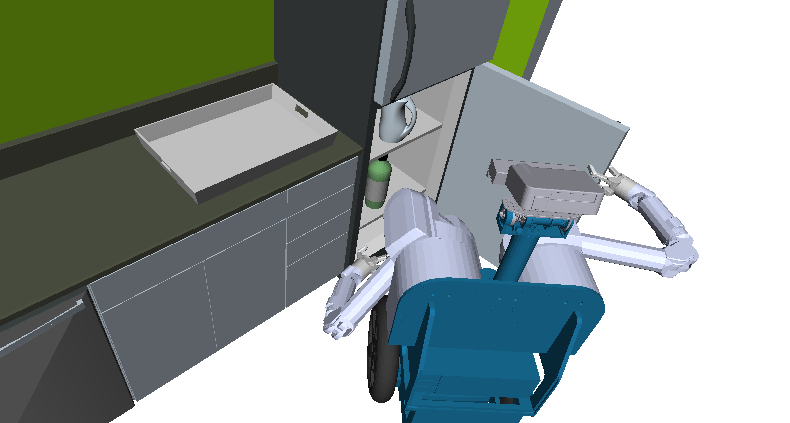
\includegraphics[width=0.2\textwidth]{figs/fridge-intro.png}%
%};

\ifdefined\drawfirstfailtraj
   \draw[red,line width=2pt] plot [smooth] coordinates {(-2,0) (1.9,1.4)};
\fi

% subset definitions
\def\crect{(-2.5,-2.5) rectangle (2.5,2.5)}
\def\bloba{(-3,1) (-1,1.5) (0,3) (3,3) (3,0.8) (-0.1,1.5) (0,1) (1,0.5) (0.5,0) (-3,-0.5)}
\def\blobb{(-3,-1) (0,-1) (3,0.5) (3,-3) (0,-2) (-3,-2)}

\ifdefined\drawcfree

   % for clipping
   \begin{scope}
      \draw[draw=none,clip,rounded corners] \crect;
      \draw[draw=none,clip] plot [smooth cycle] coordinates {\bloba};
      \draw[line width=1.5pt,rounded corners,fill=blue!20,opacity=\drawcfree] \crect;
      \draw[line width=1.5pt,opacity=\drawcfree] plot [smooth cycle] coordinates {\bloba};
   \end{scope}
   %\draw [red] plot [smooth cycle] coordinates {\bloba};
   
   \begin{scope}
      \draw[draw=none,clip,rounded corners] \crect;
      \draw[draw=none,clip] plot [smooth cycle] coordinates {\blobb};
      \draw[line width=1.5pt,rounded corners,fill=blue!20,opacity=\drawcfree] \crect;
      \draw[line width=1.5pt,opacity=\drawcfree] plot [smooth cycle] coordinates {\blobb};
   \end{scope}
   %\draw [red] plot [smooth cycle] coordinates {\blobb};
\fi
   
\ifdefined\drawcfreefuzzy

   \begin{scope}
      \draw[draw=none,clip,rounded corners] \crect;
      \draw[line width=15pt,color=blue!5] plot [smooth cycle] coordinates {\bloba};
      \draw[line width=10pt,color=blue!10] plot [smooth cycle] coordinates {\bloba};
      \draw[line width= 5pt,color=blue!15] plot [smooth cycle] coordinates {\bloba};
      \draw[draw=none,clip] plot [smooth cycle] coordinates {\bloba};
      \draw[line width=15pt,color=blue!30,fill=blue!35] plot [smooth cycle] coordinates {\bloba};
      \draw[line width=10pt,color=blue!25] plot [smooth cycle] coordinates {\bloba};
      \draw[line width= 5pt,color=blue!20] plot [smooth cycle] coordinates {\bloba};
   \end{scope}
   
   \begin{scope}
      \draw[draw=none,clip,rounded corners] \crect;
      \draw[line width=15pt,color=blue!5] plot [smooth cycle] coordinates {\blobb};
      \draw[line width=10pt,color=blue!10] plot [smooth cycle] coordinates {\blobb};
      \draw[line width= 5pt,color=blue!15] plot [smooth cycle] coordinates {\blobb};
      \draw[draw=none,clip] plot [smooth cycle] coordinates {\blobb};
      \draw[line width=15pt,color=blue!30,fill=blue!35] plot [smooth cycle] coordinates {\blobb};
      \draw[line width=10pt,color=blue!25] plot [smooth cycle] coordinates {\blobb};
      \draw[line width= 5pt,color=blue!20] plot [smooth cycle] coordinates {\blobb};
   \end{scope}

\fi
   
% draw crect itself!
\ifdefined\drawc
   \draw[rounded corners,opacity=\drawc] \crect;
   \node[opacity=\drawc] at (-2.2,2.2) {$\mathcal{C}$};
\fi

\ifdefined\argtraja
   \draw[black!30,line width=7pt,line cap=round]
      plot [smooth] coordinates {(-2,0) (2.0,1.4)};
   %\draw plot [smooth] coordinates {(-2,0) (2.0,1.4)};
\fi

\ifdefined\argrrtchosen
   \draw[black!30,line width=7pt,line cap=round]
      (-2,0) -- (-0.5,0.525) -- (-1,2) -- (1.4,1.225) -- (2.0,1.4);
\fi

% starts
\coordinate (st01) at (-2,0);
%\fill[black] (st01) circle (0.07cm);

% goals
\coordinate (go01) at (2.1,2);
\coordinate (go02) at (2.0,1.4);
\coordinate (go03) at (2.0,0.5);
\coordinate (go04) at (2.1,-0.5);
\coordinate (go05) at (1.9,-1.5);
%\fill[black] (go01) circle (0.07cm);
%\fill[black] (go02) circle (0.07cm);
%\fill[black] (go03) circle (0.07cm);
%\fill[black] (go04) circle (0.07cm);
%\fill[black] (go05) circle (0.07cm);

\ifdefined\drawpaths
   % candidate paths
   \draw[dashed] plot [smooth] coordinates {(-2,0) (0,2) (go01)};
   \draw[dashed] plot [smooth] coordinates {(-2,0) (go02)};
   \draw[dashed] plot [smooth] coordinates {(-2,0) (0.5,-0.5) (go02)};
   \draw[dashed] plot [smooth] coordinates {(-2,0) (0,0.5) (go03)};
   \draw[dashed] plot [smooth] coordinates {(-2,0) (0,-1.5) (go05)};
\fi

\ifdefined\drawtrajneighborhood
   \draw[fill=black!50,opacity=0.5] plot [smooth cycle] coordinates {(-2,0) (-0.2,1.0) (2.0,1.4) (0.2,0.4)};
   \draw plot [smooth] coordinates {(-2,0) (2.0,1.4)};
\fi

\ifdefined\argtrajd
   \draw[line width=2pt] plot [smooth] coordinates {(-2,0) (0.2,0.5) (2.0,1.4)};
\fi

\ifdefined\drawfirstfailtraj
   \begin{scope}
      \draw[draw=none,clip,rounded corners] \crect;
      \draw[draw=none,clip] plot [smooth cycle] coordinates {\bloba};
      \draw[line width=2pt] plot [smooth] coordinates {(-2,0) (2.0,1.4)};
   \end{scope}
\fi

\ifdefined\argfirstfailnext
   \draw[dashed] plot [smooth] coordinates {(-2,0) (0.2,0.9) (2.0,1.4)};
\fi

\ifdefined\drawrrtstart
   % forward tree
   \draw[line width=2pt] plot coordinates {(-2,0) (0,0.7)};
   \fill[black]
      (-1.5,0.175) circle (0.07cm)
      (-1.0,0.35) circle (0.07cm)
      (-0.5,0.525) circle (0.07cm)
      ( 0.0,0.7) circle (0.07cm);
   % forward branches
   \draw[line width=2pt] plot coordinates {(-2,0) (-1.9,0.5)};
   \fill[black] (-1.9,0.5) circle (0.07cm);
   \draw[line width=2pt] plot coordinates {(-1.0,0.35) (-0.6,0.1) (-0.1,0.1)};
   \fill[black] (-0.6,0.1) circle (0.07cm);
   \fill[black] (-0.1,0.1) circle (0.07cm);

   % reverse tree
   \draw[line width=2pt] plot coordinates {(1.4,1.225) (2.0,1.4)};
   \fill[black] (1.4,1.225) circle (0.07cm);
   % reverse branches
   \draw[line width=2pt] plot coordinates {(2.0,1.4) (1.6,1.7)};
   \fill[black] (1.6,1.7) circle (0.07cm);
   
   %\begin{scope}
   %   \draw[draw=none,clip] plot [smooth cycle] coordinates {\bloba};
   %   \draw[line width=2pt] plot [smooth] coordinates {(-2,0) (2.0,1.4)};
   %\end{scope}
\fi

\ifdefined\drawrrtcandidates
   % forward options
   \draw[dashed]
      (-2,0) -- (-1,2)
      (-1.5,0.175) -- (-1,2)
      (-1.0,0.35) -- (-1,2)
      (-0.5,0.525) -- (-1,2)
      ( 0.0,0.7) -- (-1,2)
   % branch options
      (-1.9,0.5) -- (-1,2)
      (-0.6,0.1) -- (-1,2)
      (-0.1,0.1) -- (-1,2);
      
   % reverse options
   \draw[dashed]
      (-1,2) -- (2.1,2)
      (-1,2) -- (2.0,1.4)
      (-1,2) -- (1.4,1.225)
   % branch options
      (-1,2) -- (1.6,1.7);
\fi

\ifdefined\drawrrtsample
   \fill[green] (-1,2) circle (0.07cm);
\fi

% graph stuff
\coordinate (gr01) at (-1.3, 0.2);
\coordinate (gr02) at (-0.2, 0.4);
\coordinate (gr03) at (-0.6, 1.0);
\coordinate (gr04) at (-1.7, 0.9);
\coordinate (gr05) at ( 0.6, 0.9);
\coordinate (gr06) at ( 1.2, 1.3);
\coordinate (gr07) at ( 0.3, 1.8);
\coordinate (gr08) at (-0.3, 2.0);
\coordinate (gr09) at (-1.5, 2.1);
\coordinate (gr10) at ( 1.3, 2.2);
\coordinate (gr11) at ( 1.2, 0.2);
\coordinate (gr12) at ( 0.2, 0.2);
\coordinate (gr13) at (-1.2,-0.8);
\coordinate (gr14) at (-0.6,-0.6);
\coordinate (gr15) at ( 0.4,-0.6);
\coordinate (gr16) at ( 1.1,-0.9);
\coordinate (gr17) at (-1.8,-1.2);
\coordinate (gr18) at (-1.1,-1.7);
\coordinate (gr19) at (-0.2,-1.5);
\coordinate (gr20) at ( 0.8,-1.5);
\coordinate (gr21) at (-2.0,-1.8);
\coordinate (gr22) at (-0.5,-2.2);
\coordinate (gr23) at ( 0.5,-1.9);

\ifdefined\drawgraph
   \fill[black]
      (gr01) circle (0.07cm)
      (gr02) circle (0.07cm)
      (gr03) circle (0.07cm)
      (gr04) circle (0.07cm)
      (gr05) circle (0.07cm)
      (gr06) circle (0.07cm)
      (gr07) circle (0.07cm)
      (gr08) circle (0.07cm)
      (gr09) circle (0.07cm)
      (gr10) circle (0.07cm)
      (gr11) circle (0.07cm)
      (gr12) circle (0.07cm)
      (gr13) circle (0.07cm)
      (gr14) circle (0.07cm)
      (gr15) circle (0.07cm)
      (gr16) circle (0.07cm)
      (gr17) circle (0.07cm)
      (gr18) circle (0.07cm)
      (gr19) circle (0.07cm)
      (gr20) circle (0.07cm)
      (gr21) circle (0.07cm)
      (gr22) circle (0.07cm)
      (gr23) circle (0.07cm)
      ;
   \draw[\drawgraph]
      (st01) -- (gr01) -- (gr02) -- (gr05) -- (gr06) -- (go02)
      (gr02) -- (gr03) -- (gr04) -- (gr01) -- (gr03)
      (st01) -- (gr04) -- (gr09) -- (gr03) -- (gr08) -- (gr09)
      (gr03) -- (gr05) -- (gr07) -- (gr10) -- (gr06) -- (gr07) -- (gr08)
      (gr10) -- (go01) -- (go02) -- (go03) -- (gr06)
      (gr02) -- (gr12) -- (gr05) -- (gr11) -- (go03) -- (go04)
      (gr12) -- (gr11) -- (go04) -- (go05)
      (st01) -- (gr13) -- (gr14) -- (gr15) -- (gr16) -- (go05)
      (gr13) -- (gr01) -- (gr14) -- (gr02) -- (gr15) -- (gr11)
      (gr12) -- (gr15)
      (gr13) -- (gr17) -- (gr18) -- (gr19) -- (gr20) -- (go05)
      (gr18) -- (gr13) -- (gr19) -- (gr14)
      (gr19) -- (gr15) -- (gr20) -- (gr16)
      (gr17) -- (gr21) -- (gr18) -- (gr22) -- (gr19) -- (gr23)
      (gr22) -- (gr23)  -- (gr20)
      ;
\fi

\ifdefined\arggraphfirst
   \draw
      (st01) -- (gr01) -- (gr02) -- (gr05) -- (gr06) -- (go02);
\fi

\ifdefined\arggraphfirstevaled
   \draw[red,line width=2pt] (gr02) -- (gr05) -- (gr06);
   \draw[line width=2pt]
      (st01) -- (gr01) -- (gr02) (gr06) -- (go02);
   \fill[red] (gr05) circle (0.07cm);
\fi

\ifdefined\arggraphfirstnext
   \draw[red,line width=2pt] (gr02) -- (gr05) -- (gr06);
   \draw[line width=2pt]
      (st01) -- (gr01) -- (gr02) (gr06) -- (go02);
   \fill[red] (gr05) circle (0.07cm);
   \draw
      (gr01) -- (gr03) -- (gr08) -- (gr07) -- (gr10) -- (go01);
\fi

\ifdefined\argastarb
   \draw[dashed] (st01) -- (go03);
   \fill[blue] (st01) circle (0.1cm);
\fi

\ifdefined\argastarc
   \draw[line width=2pt] (st01) -- (gr04);
   \fill[blue] (st01) circle (0.1cm);
\fi

\ifdefined\argastard
   \draw[line width=2pt] (st01) -- (gr04);
   \draw[line width=2pt] (st01) -- (gr01);
   \fill[blue] (st01) circle (0.1cm);
\fi

\ifdefined\argastare
   \draw[line width=2pt] (st01) -- (gr04);
   \draw[line width=2pt] (st01) -- (gr01);
   \draw[line width=2pt,red] (st01) -- (gr13);
   \fill[blue] (st01) circle (0.1cm);
\fi

\ifdefined\argastarf
   \draw[line width=2pt] (st01) -- (gr04);
   \draw[line width=2pt] (st01) -- (gr01);
   \draw[line width=2pt,red] (st01) -- (gr13);
   \draw[dashed] (gr01) -- (go03);
   \fill[blue] (gr01) circle (0.1cm);
\fi

\ifdefined\argastarg
   \draw[line width=2pt] (st01) -- (gr04);
   \draw[line width=2pt] (st01) -- (gr01);
   \draw[line width=2pt,red] (st01) -- (gr13);
   \draw[line width=2pt] (gr01) -- (gr04);
   \fill[blue] (gr01) circle (0.1cm);
\fi

\ifdefined\argastarh
   \draw[line width=2pt] (st01) -- (gr04);
   \draw[line width=2pt] (st01) -- (gr01);
   \draw[line width=2pt,red] (st01) -- (gr13);
   \draw[line width=2pt] (gr01) -- (gr04);
   \draw[line width=2pt] (gr01) -- (gr03);
   \fill[blue] (gr01) circle (0.1cm);
\fi

\ifdefined\argastari
   \draw[line width=2pt] (st01) -- (gr04);
   \draw[line width=2pt] (st01) -- (gr01);
   \draw[line width=2pt,red] (st01) -- (gr13);
   \draw[line width=2pt] (gr01) -- (gr04);
   \draw[line width=2pt] (gr01) -- (gr03);
   \draw[line width=2pt] (gr01) -- (gr02);
   \fill[blue] (gr01) circle (0.1cm);
\fi

\ifdefined\argastarj
   \draw[line width=2pt] (st01) -- (gr04);
   \draw[line width=2pt] (st01) -- (gr01);
   \draw[line width=2pt,red] (st01) -- (gr13);
   \draw[line width=2pt] (gr01) -- (gr04);
   \draw[line width=2pt] (gr01) -- (gr03);
   \draw[line width=2pt] (gr01) -- (gr02);
   \draw[line width=2pt,red] (gr01) -- (gr14);
   \fill[blue] (gr01) circle (0.1cm);
\fi

\ifdefined\argastark
   \draw[line width=2pt] (st01) -- (gr04);
   \draw[line width=2pt] (st01) -- (gr01);
   \draw[line width=2pt,red] (st01) -- (gr13);
   \draw[line width=2pt] (gr01) -- (gr04);
   \draw[line width=2pt] (gr01) -- (gr03);
   \draw[line width=2pt] (gr01) -- (gr02);
   \draw[line width=2pt,red] (gr01) -- (gr14);
   \draw[line width=2pt,red] (gr01) -- (gr13);
   \fill[blue] (gr01) circle (0.1cm);
\fi

\ifdefined\argastarl
   \draw[line width=2pt] (st01) -- (gr04);
   \draw[line width=2pt] (st01) -- (gr01);
   \draw[line width=2pt,red] (st01) -- (gr13);
   \draw[line width=2pt] (gr01) -- (gr04);
   \draw[line width=2pt] (gr01) -- (gr03);
   \draw[line width=2pt] (gr01) -- (gr02);
   \draw[line width=2pt,red] (gr01) -- (gr14);
   \draw[line width=2pt,red] (gr01) -- (gr13);
   % new:
   \draw[line width=2pt] (gr02) -- (gr03);
   \draw[line width=2pt,red] (gr02) -- (gr05);
   \draw[line width=2pt] (gr02) -- (gr12);
   \draw[line width=2pt,red] (gr02) -- (gr15);
   \draw[line width=2pt,red] (gr02) -- (gr14);
   \draw[dashed] (gr02) -- (go03);
   \fill[blue] (gr02) circle (0.1cm);
\fi

\ifdefined\argastarm
   \draw[line width=2pt] (st01) -- (gr04);
   \draw[line width=2pt] (st01) -- (gr01);
   \draw[line width=2pt,red] (st01) -- (gr13);
   \draw[line width=2pt] (gr01) -- (gr04);
   \draw[line width=2pt] (gr01) -- (gr03);
   \draw[line width=2pt] (gr01) -- (gr02);
   \draw[line width=2pt,red] (gr01) -- (gr14);
   \draw[line width=2pt,red] (gr01) -- (gr13);
   \draw[line width=2pt] (gr02) -- (gr03);
   \draw[line width=2pt,red] (gr02) -- (gr05);
   \draw[line width=2pt] (gr02) -- (gr12);
   \draw[line width=2pt,red] (gr02) -- (gr15);
   \draw[line width=2pt,red] (gr02) -- (gr14);
   % new:
   \draw[line width=2pt,red] (gr12) -- (gr05);
   \draw[line width=2pt,red] (gr12) -- (gr11);
   \draw[line width=2pt,red] (gr12) -- (gr15);
   \draw[dashed] (gr12) -- (go03);
   \fill[blue] (gr12) circle (0.1cm);
\fi

\ifdefined\argastarn
   \draw[line width=2pt] (st01) -- (gr04);
   \draw[line width=2pt] (st01) -- (gr01);
   \draw[line width=2pt,red] (st01) -- (gr13);
   \draw[line width=2pt] (gr01) -- (gr04);
   \draw[line width=2pt] (gr01) -- (gr03);
   \draw[line width=2pt] (gr01) -- (gr02);
   \draw[line width=2pt,red] (gr01) -- (gr14);
   \draw[line width=2pt,red] (gr01) -- (gr13);
   \draw[line width=2pt] (gr02) -- (gr03);
   \draw[line width=2pt,red] (gr02) -- (gr05);
   \draw[line width=2pt] (gr02) -- (gr12);
   \draw[line width=2pt,red] (gr02) -- (gr15);
   \draw[line width=2pt,red] (gr02) -- (gr14);
   \draw[line width=2pt,red] (gr12) -- (gr05);
   \draw[line width=2pt,red] (gr12) -- (gr11);
   \draw[line width=2pt,red] (gr12) -- (gr15);
   % new:
   \draw[line width=2pt] (gr03) -- (gr04);
   \draw[line width=2pt,red] (gr03) -- (gr09);
   \draw[line width=2pt] (gr03) -- (gr08);
   \draw[line width=2pt,red] (gr03) -- (gr05);
   \draw[dashed] (gr03) -- (go02);
   \fill[blue] (gr03) circle (0.1cm);
\fi

\ifdefined\argastaro
   \draw[line width=2pt] (st01) -- (gr04);
   \draw[line width=2pt] (st01) -- (gr01);
   \draw[line width=2pt,red] (st01) -- (gr13);
   \draw[line width=2pt] (gr01) -- (gr04);
   \draw[line width=2pt] (gr01) -- (gr03);
   \draw[line width=2pt] (gr01) -- (gr02);
   \draw[line width=2pt,red] (gr01) -- (gr14);
   \draw[line width=2pt,red] (gr01) -- (gr13);
   \draw[line width=2pt] (gr02) -- (gr03);
   \draw[line width=2pt,red] (gr02) -- (gr05);
   \draw[line width=2pt] (gr02) -- (gr12);
   \draw[line width=2pt,red] (gr02) -- (gr15);
   \draw[line width=2pt,red] (gr02) -- (gr14);
   \draw[line width=2pt,red] (gr12) -- (gr05);
   \draw[line width=2pt,red] (gr12) -- (gr11);
   \draw[line width=2pt,red] (gr12) -- (gr15);
   \draw[line width=2pt] (gr03) -- (gr04);
   \draw[line width=2pt,red] (gr03) -- (gr09);
   \draw[line width=2pt] (gr03) -- (gr08);
   \draw[line width=2pt,red] (gr03) -- (gr05);
   % new:
   \draw[line width=2pt,red] (gr04) -- (gr09);
   \draw[dashed] (gr04) -- (go03);
   \fill[blue] (gr04) circle (0.1cm);
\fi

\ifdefined\argastarp
   \draw[line width=2pt] (st01) -- (gr04);
   \draw[line width=2pt] (st01) -- (gr01);
   \draw[line width=2pt,red] (st01) -- (gr13);
   \draw[line width=2pt] (gr01) -- (gr04);
   \draw[line width=2pt] (gr01) -- (gr03);
   \draw[line width=2pt] (gr01) -- (gr02);
   \draw[line width=2pt,red] (gr01) -- (gr14);
   \draw[line width=2pt,red] (gr01) -- (gr13);
   \draw[line width=2pt] (gr02) -- (gr03);
   \draw[line width=2pt,red] (gr02) -- (gr05);
   \draw[line width=2pt] (gr02) -- (gr12);
   \draw[line width=2pt,red] (gr02) -- (gr15);
   \draw[line width=2pt,red] (gr02) -- (gr14);
   \draw[line width=2pt,red] (gr12) -- (gr05);
   \draw[line width=2pt,red] (gr12) -- (gr11);
   \draw[line width=2pt,red] (gr12) -- (gr15);
   \draw[line width=2pt] (gr03) -- (gr04);
   \draw[line width=2pt,red] (gr03) -- (gr09);
   \draw[line width=2pt] (gr03) -- (gr08);
   \draw[line width=2pt,red] (gr03) -- (gr05);
   \draw[line width=2pt,red] (gr04) -- (gr09);
   % new:
   \draw[line width=2pt,red] (gr08) -- (gr09);
   \draw[line width=2pt] (gr08) -- (gr07);
   \draw[dashed] (gr08) -- (go01);
   \fill[blue] (gr08) circle (0.1cm);
\fi

\ifdefined\argastarq
   \draw[line width=2pt] (st01) -- (gr04);
   \draw[line width=2pt] (st01) -- (gr01);
   \draw[line width=2pt,red] (st01) -- (gr13);
   \draw[line width=2pt] (gr01) -- (gr04);
   \draw[line width=2pt] (gr01) -- (gr03);
   \draw[line width=2pt] (gr01) -- (gr02);
   \draw[line width=2pt,red] (gr01) -- (gr14);
   \draw[line width=2pt,red] (gr01) -- (gr13);
   \draw[line width=2pt] (gr02) -- (gr03);
   \draw[line width=2pt,red] (gr02) -- (gr05);
   \draw[line width=2pt] (gr02) -- (gr12);
   \draw[line width=2pt,red] (gr02) -- (gr15);
   \draw[line width=2pt,red] (gr02) -- (gr14);
   \draw[line width=2pt,red] (gr12) -- (gr05);
   \draw[line width=2pt,red] (gr12) -- (gr11);
   \draw[line width=2pt,red] (gr12) -- (gr15);
   \draw[line width=2pt] (gr03) -- (gr04);
   \draw[line width=2pt,red] (gr03) -- (gr09);
   \draw[line width=2pt] (gr03) -- (gr08);
   \draw[line width=2pt,red] (gr03) -- (gr05);
   \draw[line width=2pt,red] (gr04) -- (gr09);
   \draw[line width=2pt,red] (gr08) -- (gr09);
   \draw[line width=2pt] (gr08) -- (gr07);
   % new:
   \draw[line width=2pt] (gr07) -- (gr10);
   \draw[line width=2pt] (gr07) -- (gr06);
   \draw[line width=2pt,red] (gr07) -- (gr05);
   \draw[dashed] (gr07) -- (go01);
   \fill[blue] (gr07) circle (0.1cm);
\fi

\ifdefined\argastarr
   \draw[line width=2pt] (st01) -- (gr04);
   \draw[line width=2pt] (st01) -- (gr01);
   \draw[line width=2pt,red] (st01) -- (gr13);
   \draw[line width=2pt] (gr01) -- (gr04);
   \draw[line width=2pt] (gr01) -- (gr03);
   \draw[line width=2pt] (gr01) -- (gr02);
   \draw[line width=2pt,red] (gr01) -- (gr14);
   \draw[line width=2pt,red] (gr01) -- (gr13);
   \draw[line width=2pt] (gr02) -- (gr03);
   \draw[line width=2pt,red] (gr02) -- (gr05);
   \draw[line width=2pt] (gr02) -- (gr12);
   \draw[line width=2pt,red] (gr02) -- (gr15);
   \draw[line width=2pt,red] (gr02) -- (gr14);
   \draw[line width=2pt,red] (gr12) -- (gr05);
   \draw[line width=2pt,red] (gr12) -- (gr11);
   \draw[line width=2pt,red] (gr12) -- (gr15);
   \draw[line width=2pt] (gr03) -- (gr04);
   \draw[line width=2pt,red] (gr03) -- (gr09);
   \draw[line width=2pt] (gr03) -- (gr08);
   \draw[line width=2pt,red] (gr03) -- (gr05);
   \draw[line width=2pt,red] (gr04) -- (gr09);
   \draw[line width=2pt,red] (gr08) -- (gr09);
   \draw[line width=2pt] (gr08) -- (gr07);
   \draw[line width=2pt] (gr07) -- (gr10);
   \draw[line width=2pt] (gr07) -- (gr06);
   \draw[line width=2pt,red] (gr07) -- (gr05);
   % new:
   \draw[line width=2pt] (gr10) -- (go01);
   \draw[line width=2pt] (gr10) -- (gr06);
   \draw[dashed] (gr10) -- (go01);
   \fill[blue] (gr10) circle (0.1cm);
\fi

\ifdefined\argastars
   \draw[line width=2pt] (st01) -- (gr04);
   \draw[line width=2pt] (st01) -- (gr01);
   \draw[line width=2pt,red] (st01) -- (gr13);
   \draw[line width=2pt] (gr01) -- (gr04);
   \draw[line width=2pt] (gr01) -- (gr03);
   \draw[line width=2pt] (gr01) -- (gr02);
   \draw[line width=2pt,red] (gr01) -- (gr14);
   \draw[line width=2pt,red] (gr01) -- (gr13);
   \draw[line width=2pt] (gr02) -- (gr03);
   \draw[line width=2pt,red] (gr02) -- (gr05);
   \draw[line width=2pt] (gr02) -- (gr12);
   \draw[line width=2pt,red] (gr02) -- (gr15);
   \draw[line width=2pt,red] (gr02) -- (gr14);
   \draw[line width=2pt,red] (gr12) -- (gr05);
   \draw[line width=2pt,red] (gr12) -- (gr11);
   \draw[line width=2pt,red] (gr12) -- (gr15);
   \draw[line width=2pt] (gr03) -- (gr04);
   \draw[line width=2pt,red] (gr03) -- (gr09);
   \draw[line width=2pt] (gr03) -- (gr08);
   \draw[line width=2pt,red] (gr03) -- (gr05);
   \draw[line width=2pt,red] (gr04) -- (gr09);
   \draw[line width=2pt,red] (gr08) -- (gr09);
   \draw[line width=2pt] (gr08) -- (gr07);
   \draw[line width=2pt] (gr07) -- (gr10);
   \draw[line width=2pt] (gr07) -- (gr06);
   \draw[line width=2pt,red] (gr07) -- (gr05);
   \draw[line width=2pt] (gr10) -- (go01);
   \draw[line width=2pt] (gr10) -- (gr06);
   % new:
   \fill[blue] (go01) circle (0.1cm);
\fi

% draw starts and goals
\node[draw,circle,inner sep=2pt,ultra thick,fill=red!50] at (st01) {};
\node[draw,circle,inner sep=2pt,ultra thick,fill=green!50] at (go01) {};
\node[draw,circle,inner sep=2pt,ultra thick,fill=green!50] at (go02) {};
\node[draw,circle,inner sep=2pt,ultra thick,fill=green!50] at (go03) {};
\node[draw,circle,inner sep=2pt,ultra thick,fill=green!50] at (go04) {};
\node[draw,circle,inner sep=2pt,ultra thick,fill=green!50] at (go05) {};

%\draw[step=1,black!10,very thin] (-2,-2) grid (2,2);
   
\end{tikzpicture}%
\end{document}%
